\section{Tutorial -- ACOSSO}
\label{(sec.surrogate.acosso)}

This tutorial covers the ACOSSO surrogate modeling method. The Adaptive
COmponent Selection and Shrinkage Operator (ACOSSO) surface approximation
was developed under the Smoothing Spline Analysis of Variance (SS-ANOVA)
modeling framework \citep{Storlie_2011}. As it is a smoothing type method,
ACOSSO works best when the underlying function is somewhat smooth. For
functions which are known to have sharp changes or peaks, etc., other
methods may be more appropriate. Since it implicitly performs variable
selection, ACOSSO can also work well when there are a large number of input
variables. 
The ACOSSO procedure also allows for
categorical inputs \citep{Storlie_2013}.
 
This tutorial uses the same flowsheet and sample setup as the ALAMO
tutorial in Section \ref{sec.surrogate.alamo}. The statistics software
``R'' is also required to use ACOSSO and BSS-ANOVA. Before starting this
tutorial, you will need to install R version 3.1 or later (see \href{http://cran.r-project.org/}{\textcolor{blue}{https://cran.r-project.org/}}). 

Once R is installed, you will need to install the ``quadprog''
package. ACOSSO requires this package for solving quadratic
programming problems. You will only need to perform this step once. 

\begin{enumerate}
\item{Start R. In Windows, this must be done with administrative
  privileges.  Either run this from an administrator account, or
  right-click ``R x64 3.1.2'' and click ``Run with administrator'' and type
  in administrator credentials.}
\item{Inside the R console, type:
   \begin{itemize} 
   \item \tt install.packages('quadprog')
   \item \tt library(quadprog)
   \item \tt q()
  \end{itemize}
The first line installs the package. If prompted for a CRAN mirror, select
the one closest to you geographically. The second line loads the
package. The last line quits R. If prompted to save workspace image, choose
`y'.}
\end{enumerate}

Once you have done these steps, ACOSSO is ready to be invoked inside FOQUS.

\begin{enumerate}
	\item{Set the path to the RScript executable.}
		\begin{enumerate}
			\item Click the \bu{Settings} button in the Home window.
			\item Change the RScript path if necessary. The \bu{Browse} button
           opens a file browser that can be used to set the path.
		\end{enumerate}
	\item Complete the ALAMO tutorial in Section \ref{sec.surrogate.alamo} through Step 32, or load the FOQUS session saved after completing the ALAMO tutorial.
	\item Click the \bu{Surrogates} button in the Home window (Figure \ref{fig.acosso.settings}).
	\item Select ``ACOSSO'' in the \bu{Tool} drop-down list.
	\item Select the \bu{Method Settings} tab.
	\item Set ``Data Filter'' to ``Initial.''
	\item Set ``Use Flowsheet Data'' to ``Yes.''
	\item Set ``FOQUS Model (for UQ)'' to ``ACOSSO\_Tutorial\_UQ.py.''
	\item Set ``FOQUS Model (for Flowsheet)'' to ``ACOSSO\_Tutorial\_FS.py.''
	\item Click the \bu{Run} icon (Figure \ref{fig.acosso.settings}).
\end{enumerate}

\begin{figure}[H]
	\begin{center}
		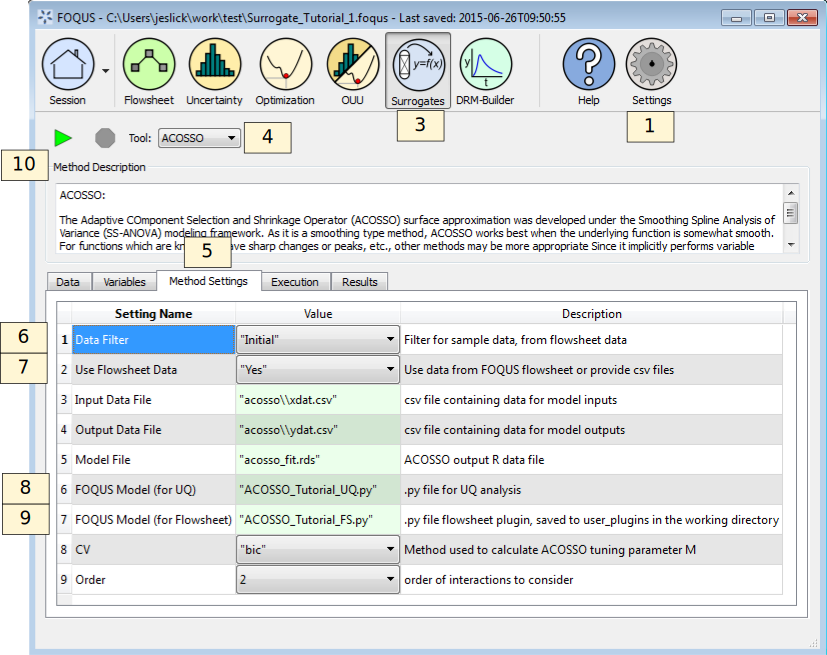
\includegraphics[scale=0.55]{Chapt_surrogates/figs/acosso_settings}
		\caption{ACOSSO Session Set Up}
		\label{fig.acosso.settings}
	\end{center}
\end{figure}

\begin{enumerate}
	\setcounter{enumi}{10}
	\item The execution window will automatically display. While ACOSSO is
     running, the execution window may show warnings, but this is normal.
	\item When the run completes, a UQ driver file is created, allowing the
     ACOSSO surrogate to be used as a user-defined response surface in UQ
     analyses. (See Section \ref{tutorial.surrogate.uq}.)
	\item ACOSSO also produces a flowsheet plugin; however.
\end{enumerate}


